% Sablon pentru realizarea lucrarii de licenta, conform cu recomandarile
% din ghidul de redactare:
% - https://fmi.unibuc.ro/finalizare-studii/

% Multumiri lui Gabriel Majeri, acest sablon a fost creat pe baza
% codului sursa a lucrarii sale de licenta. 
% Codul sursa: https://github.com/GabrielMajeri/bachelors-thesis
% Website: https://www.gabrielmajeri.ro/
%
% Acest sablon este licentiat sub Creative Commons Attribution 4.0 International License.
% modificat 8 noiembrie 2024

\documentclass[12pt, a4paper]{report}

% Suport pentru diacritice și alte simboluri
\usepackage{fontspec}

% Font Times New Roman
\usepackage{times}

% Suport pentru mai multe limbi
\usepackage{polyglossia}

% Setează limba textului la română
\setdefaultlanguage{romanian}
% Am nevoie de engleză pentru rezumat
\setotherlanguages{english}

% Indentează și primul paragraf al fiecărei noi secțiuni
\SetLanguageKeys{romanian}{indentfirst=true}

% Suport pentru diferite stiluri de ghilimele
\usepackage{csquotes}

\DeclareQuoteStyle{romanian}
  {\quotedblbase}
  {\textquotedblright}
  {\guillemotleft}
  {\guillemotright}

% Utilizează biblatex pentru referințe bibliografice
\usepackage[
    maxbibnames=50,
    sorting=nty
]{biblatex}

\addbibresource{bibliography.bib}

% Setează spațiere inter-linie (doublespacing din LaTeX este echivalentul setarii 1.5 in Microsoft Word)
\usepackage{setspace}
\doublespacing

% Modificarea geometriei paginii (cu margini de 2,5 cm) 
\usepackage[margin=2.5cm]{geometry}

% Include funcțiile de grafică
\usepackage{graphicx}
% Încarcă imaginile din directorul `images`
\graphicspath{{./images/}}

% Listări de cod
\usepackage{listings}

% Linkuri interactive în PDF
\usepackage[
    colorlinks,
    linkcolor={black},
    menucolor={black},
    citecolor={black},
    urlcolor={blue}
]{hyperref}

% Simboluri matematice codificate Unicode
\usepackage[warnings-off={mathtools-colon,mathtools-overbracket}]{unicode-math}

% Comenzi matematice
\usepackage{amsmath}
\usepackage{mathtools}

% Formule matematice
\newcommand{\bigO}[1]{\mathcal{O}\left(#1\right)}
\DeclarePairedDelimiter\abs{\lvert}{\rvert}

% Suport pentru rezumat în două limbi
% Bazat pe https://tex.stackexchange.com/a/70818
\newenvironment{abstractpage}
  {\cleardoublepage\vspace*{\fill}\thispagestyle{empty}}
  {\vfill\cleardoublepage}
\renewenvironment{abstract}[1]
  {\bigskip\selectlanguage{#1}%
   \begin{center}\bfseries\abstractname\end{center}}
  {\par\bigskip}

% Suport pentru anexe
\usepackage{appendix}

% Stiluri diferite de headere și footere
\usepackage{fancyhdr}

% Metadate
\title{FARM DEFENSE HARVEST WARS}
\author{Țacu Darius-Ștefan}

% Generează variabilele cu @
\makeatletter

\begin{document}

% Front matter
\cleardoublepage
\let\ps@plain

% Pagina de titlu
\include{0-title}
\restoregeometry
\newgeometry{
  margin=2.5cm
}

\fancypagestyle{main}{
  \fancyhf{}
  \renewcommand\headrulewidth{0pt}
  \fancyhead[C]{}
  \fancyfoot[C]{\thepage}
}

\addtocounter{page}{1}

% Rezumatul
\begin{abstractpage}

    \begin{abstract}{romanian}
        Prezenta lucrare descrie proiectarea și implementarea jocului \textit{Farm Defense: Harvest Wars}, un joc multiplayer PvP din categoria \textit{Tower Defense} cu logică de joc asimetrică. Sistemul elimină vulnerabilitățile rețelelor \textit{Peer-to-Peer} implementând o arhitectură strict \textit{Server-Authoritative}. Clientul este dezvoltat în Godot 4.x, iar backend-ul este construit cu ASP.NET Core, utilizând SQLite și Entity Framework Core pentru persistența datelor. Prin testare s-a validat un mecanism de \textit{debouncing} asincron ce reduce traficul HTTP cu până la cu 90\%, alături de un algoritm de matchmaking \textit{thread-safe} capabil de orchestrarea tranzacțiilor atomice trafic intens, garantând integritatea jocului.
    \end{abstract}

    \begin{abstract}{english}
        This thesis describes the design and implementation of \textit{Farm Defense: Harvest Wars}, a PvP \textit{Tower Defense} multiplayer game with asymmetric gameplay.
        The system mitigates \textit{Peer-to-Peer} vulnerabilities by enforcing a strict \textit{Server-Authoritative} architecture. The client is developed using Godot 4.x, while the backend is built with ASP.NET Core, utilizing SQLite and Entity Framework Core for data persistence. Tests validated an asynchronous client-side \textit{debouncing} mechanism that reduces HTTP traffic by up to 90\%, alongside a \textit{thread-safe} matchmaking algorithm capable of orchestrating atomic transactions under heavy load, ensuring complete game state integrity.
    \end{abstract}

\end{abstractpage}

\tableofcontents

% Main matter
\cleardoublepage
\pagestyle{main}
\let\ps@plain\ps@main

% Capitolul 1: Introducere
\chapter{Introducere}
\label{ch:introducere}

\section{Contextul și motivația lucrării}
În procesul dezvoltării jocurilor de strategie multiplayer în timp real se întâmpină provocări critice: menținerea unei stări de joc sincronizate și minimizarea latenței. Motivația proiectului \textit{Farm Defense: Harvest Wars} pornește de la absența pe piață a unui titlu competitiv de tipul \textit{Tower Defense} cu gameplay de asimetrie totală (unde un jucător este exclusiv atacator, iar celălalt exclusiv apărător). Soluția propusă combină acest tip de \textit{gameplay} cu o arhitectură tehnică modernă: izolarea proceselor, scalabilitate concurentă și decuplarea UI-ului de un server autoritar, prevenindu-se astfel desincronizările și manipularea datelor în scop malițios, lipsit de fair-play (\textit{cheating}).

\section{Stadiul actual al domeniului (Related Work)}
Analiza industriei evidențiază un compromis constant între mecanicile asimetrice și sistemele de progresie. De exemplu, \textit{Plants vs. Zombies} a standardizat deplasarea liniară pe benzi și gestionarea eficientă a economiei interne (\textit{in-game resource management} pentru plasarea unităților), dar rămâne o experiență strict \textit{single-player} (PvE). Pe de altă parte, \textit{Clash Royale} excelează printr-un \textit{metagame} competitiv atractiv, introducând o progresie persistentă a pachetelor de unități în afara meciurilor, spre deosebire de resetarea specifică jocurilor de tip MOBA (ex. \textit{League of Legends}). Totuși, titlurile PvP populare (inclusiv \textit{Bloons TD Battles 2}) forțează o mecanică \textit{simetrică}, în care ambii jucători atacă și se apără simultan pe aceeași arenă.

Lucrarea de față integrează economia dinamică pe benzi și progresia persistentă a unităților într-un mediu PvP competitiv cu asimetrie totală. Pentru a susține tehnic acest sistem de \textit{metagame} și a preveni manipularea progresiei sau a resurselor economice prin rețele nesigure \textit{Peer-to-Peer} (P2P), proiectul implementează o arhitectură \textit{Server-Authoritative} strictă, validată centralizat.

\section{Obiectivele proiectului}
Pentru a soluționa provocările identificate, lucrarea urmărește trei obiective arhitecturale principale:
\begin{enumerate}
    \item \textbf{Model Server-Authoritative strict:} Izolarea logicii decizionale în instanțe de joc \textit{Godot Headless}, garantând că backend-ul este singurul arbitru al stării jocului și al economiei.
    \item \textbf{Matchmaking rezilient:} Construirea unui algoritm tranzacțional atomic, capabil să proceseze concurent cererile jucătorilor, eliminând coliziunile de memorie (\textit{race conditions}).
    \item \textbf{Sincronizare asincronă non-blocantă:} Proiectarea unui mecanism de \textit{debouncing} pe client care elimină suprasolicitarea rețelei (\textit{spamming} HTTP) și maschează latența.
\end{enumerate}

\textit{Notă privind structura lucrării: Teza este organizată astfel încât să reflecte fluxul decizional tehnic: Capitolul 2 justifică ecosistemul tehnologic ales, Capitolul 3 detaliază arhitectura sistemului distribuit, Capitolul 4 analizează algoritmii concurenți de matchmaking, iar Capitolul 5 validează empiric eficiența și siguranța soluției propuse.}

% Capitolul 2: Tehnologii Utilizate
\chapter{Tehnologii Utilizate}
\label{ch:tehnologii}

Dezvoltarea proiectului \textit{Farm Defense: Harvest Wars} a necesitat o selecție riguroasă a tehnologiilor, având ca obiectiv performanța ridicată, portabilitatea și un ciclu de dezvoltare eficient. Această secțiune detaliază ecosistemul software utilizat, argumentând alegerile tehnice făcute.

\section{Motorul de joc Godot 4.x}
\label{sec:godot}

Pentru partea de client (Game Client), a fost ales motorul de joc Godot Engine, versiunea 4.x \cite{godot_docs}. Godot este un motor \textit{open-source} care oferă o arhitectură bazată pe noduri și scene, fiind extrem de flexibil pentru jocuri 2D și 3D. 

Principalele motive pentru alegerea acestui motor sunt:
\begin{itemize}
    \item \textbf{Suport C\# nativ:} Permite utilizarea unui limbaj de programare modern și performant, comun cu cel utilizat pe server.
    \item \textbf{Sistem de animație procedurală:} Facilitate esențială pentru mișcarea fluidă a unităților.
    \item \textbf{Performanță și mărime redusă:} Motorul este optimizat pentru execuție rapidă și are o amprentă mică pe disc, facilitând distribuția.
\end{itemize}

\section{Ecosistemul .NET și Limbajul C\#}
\label{sec:dotnet}

Întregul sistem (atât clientul, cât și serverul) este dezvoltat folosind limbajul C\# (versiunea 10 și ulterioare) pe platforma .NET \cite{csharp_nutshell}. Utilizarea unui limbaj unic pe ambele părți ale aplicației a permis partajarea modelelor de date (Shared Models) și a redus timpul necesar context-switch-ului între limbaje diferite.

Serverul este implementat folosind ASP.NET Core \cite{aspnet_docs}, beneficiind de performanțele ridicate ale acestui framework în gestionarea cererilor HTTP și a proceselor de fundal necesare matchmaking-ului.

\section{Gestiunea Datelor: SQLite și Entity Framework Core}
\label{sec:sqlite_ef}

Pentru persistența datelor la nivel de server, s-a optat pentru SQLite \cite{sqlite_docs}, un motor de baze de date relaționale \textit{serverless}, integrat direct în aplicație. SQLite este ideal pentru acest proiect datorită simplității în configurare și portabilității bazei de date sub formă de fișier unic.

Interacțiunea cu baza de date este realizată prin intermediul \textit{Object-Relational Mapper}-ului (ORM) Entity Framework Core \cite{ef_core_action}. S-a utilizat abordarea \textit{Code-First}, care permite definirea structurii bazei de date direct prin clase C\# și gestionarea evoluției schemei prin migrații controlate.

\section{Mediul de Dezvoltare și Operare: Ubuntu și Linux}
\label{sec:os}

Atât mediul de dezvoltare, cât și cel de operare pentru server, sunt bazate pe sistemul de operare Ubuntu Linux. Stabilitatea și securitatea oferite de nucleul Linux, împreună cu performanța ridicată a runtime-ului .NET pe această platformă, au asigurat un mediu de lucru robust pentru întregul ciclu de viață al proiectului.


% Capitolul 3: Arhitectura Sistemului
\chapter{Arhitectura Sistemului}
\label{ch:arhitectura}

În procesul dezvoltării sistemului software pentru proiectul \textit{Farm Defense: Harvest Wars}, a fost esențială utilizarea unor șabloane de proiectare (design patterns) consacrare și a
unei arhitecturi bine structurate. Arhitectura aleasă asigură separarea responsabilităților și mentenabilitatea pe termen lung a codului.

\section{Arhitectura Generală a Sistemului (Modelul C4)}
\label{sec:arhitectura_sistem}

Pentru a vizualiza arhitectura sistemului distribuit \textit{Farm Defense: Harvest Wars}, a fost utilizat modelul C4 \cite{brown_c4_model} la nivelul 2, diagramă de containere (Container Level). Modelul C4 a fost creat de Simon Brown ca o alternativă modernă la diagrama clasică UML. Avantajele sale includ simplitatea și claritatea reprezentării arhitecturii software. În acest caz, sistemul este structurat precum un model client-server, unde exista decuplare clară între logica de business și faza de gameplay în timp real.

În figura \ref{fig:c4_container}, se observă arhitectura formată din 4 containere principale:
\begin{enumerate}
    \item \textbf{Godot Game Client:} Reprezintă aplicația ce există pe computerul utilizatorului. Prin intermediul ei ultilizatorul interacționează atât cu logica din meniu (ex: selectarea unităților, deschidera cutiilor de recompense etc.), cât și cu faza de gameplay în timp real (ex: plasarea unităților etc.)
    \item \textbf{ASP.NET Core Backend:} Funcționează ca un REST API și ca un orchestrator de instanțe de joc. Acesta validează autentificarea utilizatorilor prin sistemul Identity, procesează tranzacțiile de tip metagame (modificarea pachetelor de unități) și rulează algoritmul de matchmaking.
    \item \textbf{Baza de Date SQLite:}
          Asigură stratul de persistență a datelor, comunicarea este abstractizată prin pachetul \textbf{Entity Framework Core}, care oferă un model de programare orientat pe obiecte.
    \item \textbf{Godot Headless Servers (Servere Dedicate):} Când se formează un meci valid, backend-ul execută un nou proces Godot rulat în mod \textit{headless} (fără interfață grafică), câruia îi sunt transmise datele despre meci si jucatori(id-ul meciului, unitătile selectate de jucatori etc.). Clientul primește datele meciului pentru a se putea conecta direct la acest server dedicat pentru faza de \textit{gameplay}.
\end{enumerate}

Această abordare micro-arhitecturală previne blocajele (bottlenecks) la nivelul API-ului web și izolează logic fiecare meci în propriul proces alocat de sistemul de operare Linux.

\begin{figure}[htbp]
    \centering
    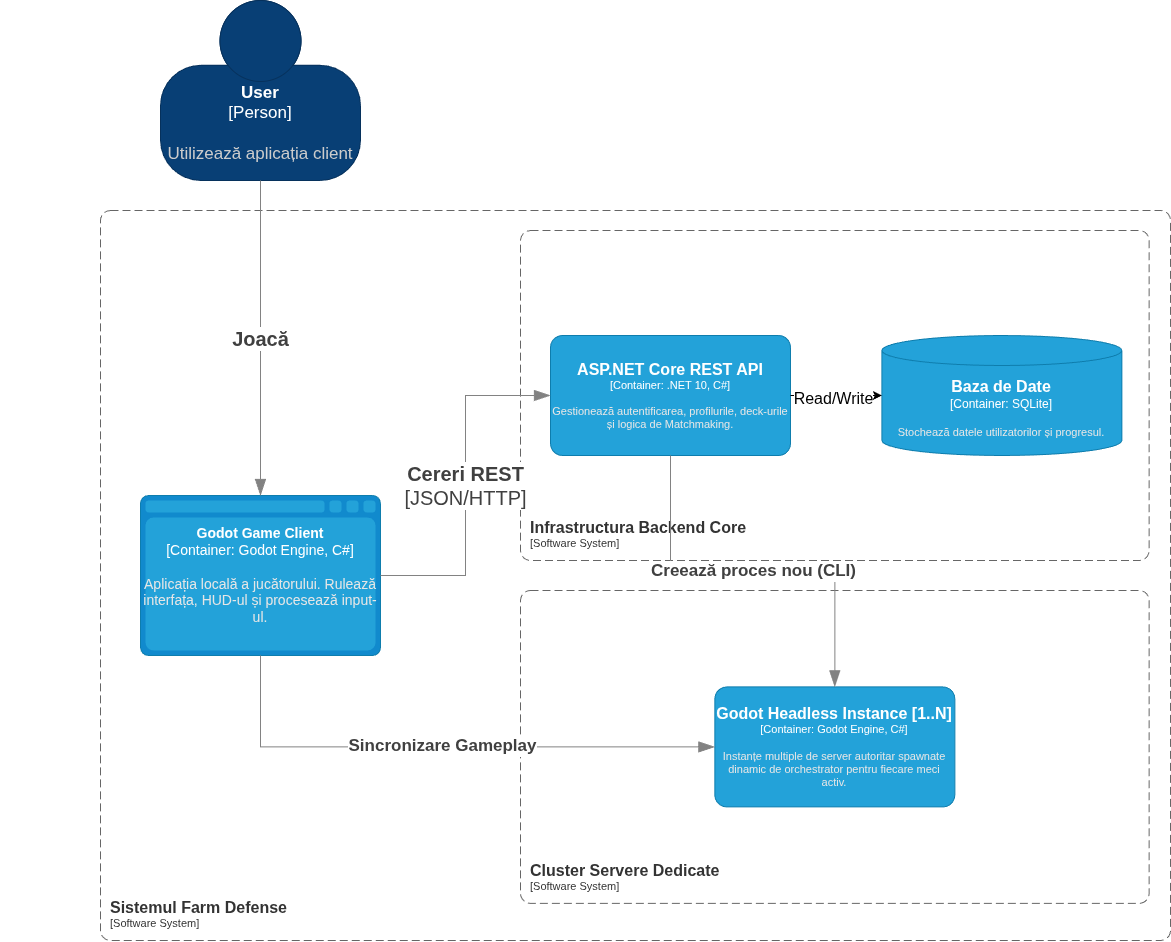
\includegraphics[width=0.7\textwidth]{DiagramaC4.png}

    \caption{Diagrama de Arhitectură C4 (Nivel Container)}
    \label{fig:c4_container}
\end{figure}

\section{Arhitectura Clientului (Godot Engine)}
\label{sec:arhitectura_client}

Clientul este construit arhitectural pe principiul modularității. Principalul design pattern utilizat este \textit{Component Pattern}\cite{nystrom_game_patterns}, adaptat la specificul motorului de joc Godot. În loc să folosim clase monolitice pentru unitățile de joc, am optat pentru o compoziție de noduri copii specializate.


\subsection{Șablonul Component (Component Pattern)}

Fiecare unitate (ex: \textit{ChickenUnit}) este un ansamblu de componente independente precum \texttt{HitboxComponent}, \texttt{HealthComponent} și \texttt{UnitStateMachine}. Această abordare permite atât reutilizarea codului cât și testarea fiecărei funcționalități în mod independent.


\begin{figure}[htbp]
    \centering
    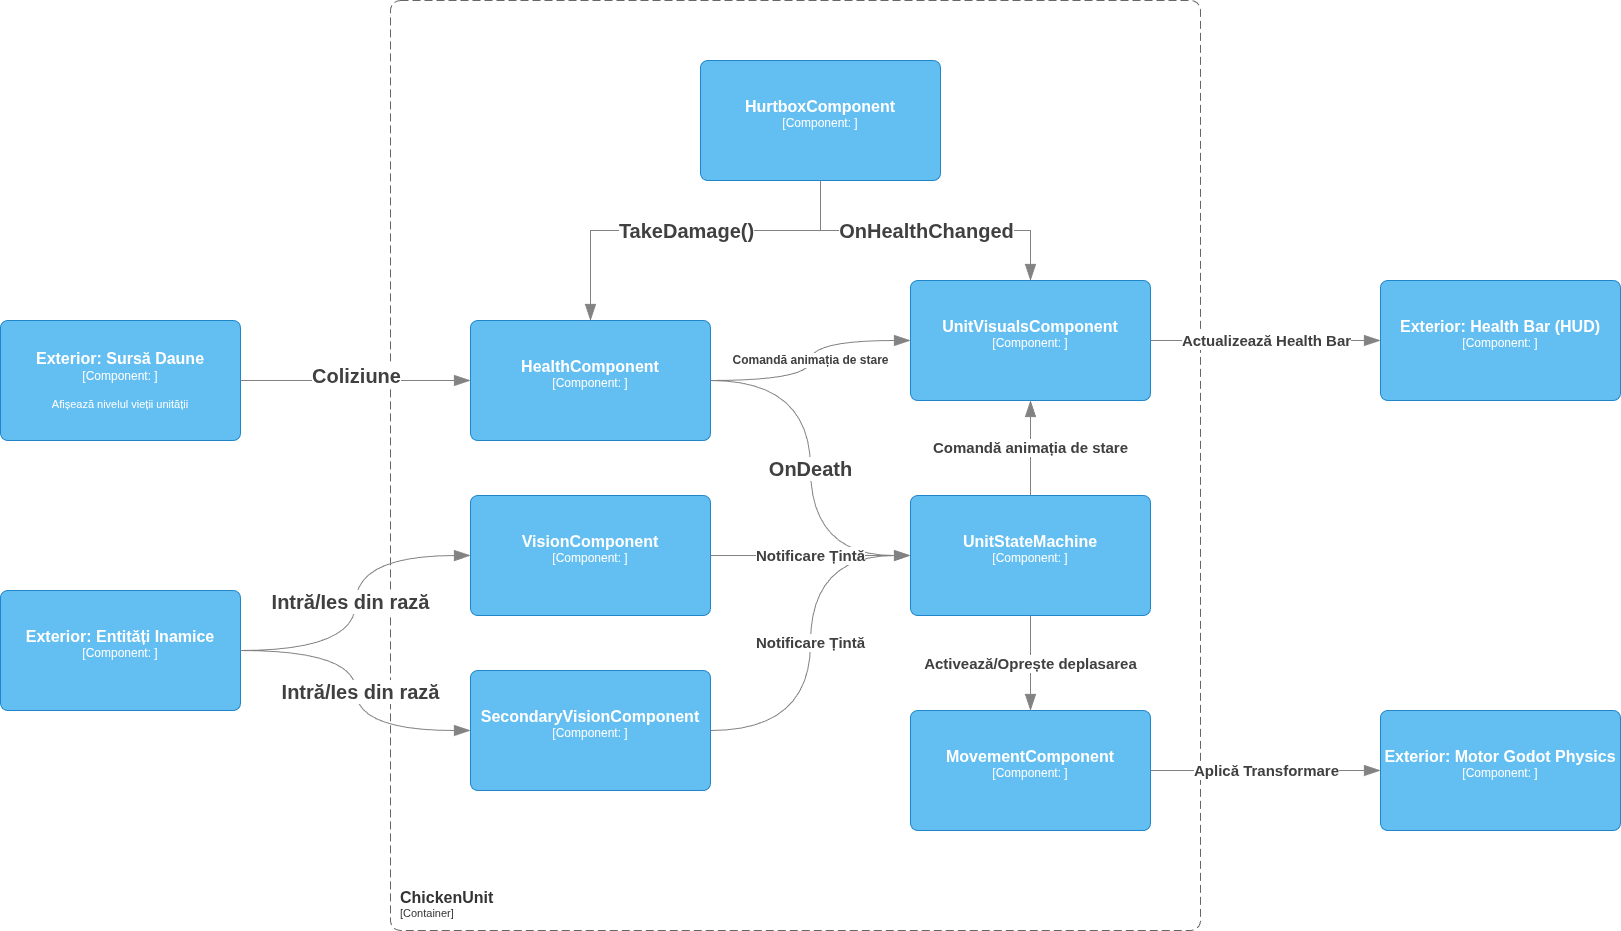
\includegraphics[width=0.9\textwidth]{ChickenC4Component.png}
    \caption{Diagrama de Componente a unei Unități, nivel Component \cite{brown_c4_model}}
    \label{fig:diagrama_componente}
\end{figure}

Pe baza arhitecturii ilustrate, responsabilitățile din entitatea \textit{ChickenUnit} au fost împărțite, conform principiului SRP (Single Responsibility Principle) \cite{martin2003agile}, în următoarele componente:

\begin{itemize}
    \item \textbf{\texttt{UnitStateMachine}:} Reprezintă componenta care orchestrează tranzițiile între stările de idle, move, attack și die.
    \item \textbf{\texttt{HealthComponent} și \texttt{HurtboxComponent}:} Gestionează variabila de viață a unei unități și validează coliziunile fizice ce au rol în aplicarea daunelor.
    \item \textbf{\texttt{VisionComponent} (Principal și Secundar):} Acționează ca senzori pentru a detecta unitățile inamice. Unitățile Defender au doi senzori de viziune: unul în partea stângă și unul în partea dreaptă.
    \item \textbf{\texttt{UnitVisualsComponent}:} Funcționează pe bază de evenimente (semnale), ascultând schimbările de stare și actualizează animațiile și HUD-ul (Health Bar).
\end{itemize}

\subsection{Șablonul Stare (State Pattern)}
\label{sec:state_pattern}

Comportamentul unităților de joc a fost modelat în principiu folosind șablonul de proiectare Stare (State Pattern) \cite{gof_design_patterns}. De regulă, în cadrul unui joc de tip strategie, o unitate oscilează constant între diverse stări: repaus, deplasare sau atac. Abordarea naivă pentru modelarea acestui tip de comportament presupune utilizarea unor structuri condiționale masive (ex. instrucțiuni \texttt{switch} sau \texttt{if-else} înlănțuite) în cadrul loop-ului principal de actualizare (\texttt{\_PhysicsProcess} în Godot). Această tip de abordare duce rapid la o degradare a gestionării codului, încălcând principiul de responsabilitate unică (Single Responsibility Principle).

Soluția este implementată cu ajutorul clasei \texttt{UnitStateMachine}, care permite decuplarea logicii fiecărui comportament. Starea este reprezentată de o singură clasă separată care implementează interfața \texttt{IState}.

În acest caz particular, sunt definite trei comportamente(\ref{fig:state_transition}) de bază pentru unități, fiecare comportament fiind reprezentat de o clasă specifică:

% --- PLACEHOLDER DIAGRAMA TRANZIȚIE STĂRI ---
\begin{figure}[htbp]
    \centering
    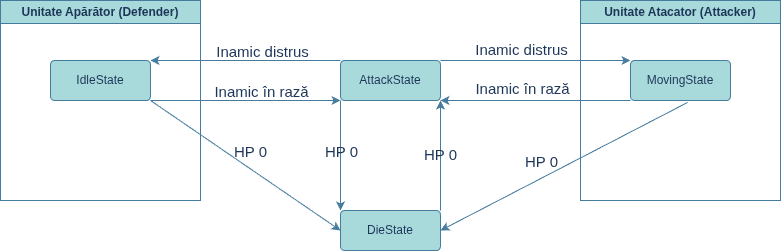
\includegraphics[width=1\textwidth]{StateDiagram.png}
    \caption{Diagrama de tranziție a stărilor pentru unități}
    \label{fig:state_transition}
\end{figure}
% --------------------------------------------

\begin{itemize}
    \item \textbf{IdleState:} Gestionează starea în care unitatea este în repaus și scanează mediul pentru detectarea țintelor cu ajutorul componentei de viziune.
    \item \textbf{MovingState:} Controlează deplasarea în direcția bazei inamice sau către o unitate inamică.
    \item \textbf{AttackState:} Reprezintă componenta de luptă, este declanșată când o unitate inamică intră în raza de viziune.
\end{itemize}

\subsubsection{Specializarea stărilor prin Interfețe Derivate (Polimorfism)}
\label{sec:state_inheritance}

Pentru a nu duplica logica și pentru a gestiona moduri diferite de atac (atacatori corp-la-corp vs. atacatori la distanță), s-a recurs la implementarea unei ierarhii de tipuri bazată pe interfețe.

S-a introdus interfața \texttt{IAttackState}, care acționează ca o interfață marcaj (marker interface) și extinde interfața de bază \texttt{IState}. Aceasta definește contractul strict pentru orice secvență de luptă, expunând timpii de pregătire (\texttt{WindUpTimer}), de reîncărcare (\texttt{CooldownTimer}) și metoda declanșatoare \texttt{StartAttackSequence()}.
Arhitectura claselor care implementează acest sistem este detaliată în Figura \ref{fig:uml_attack_state}.

% --- PLACEHOLDER DIAGRAMA UML CLASE ---
\begin{figure}[htbp]
    \centering
    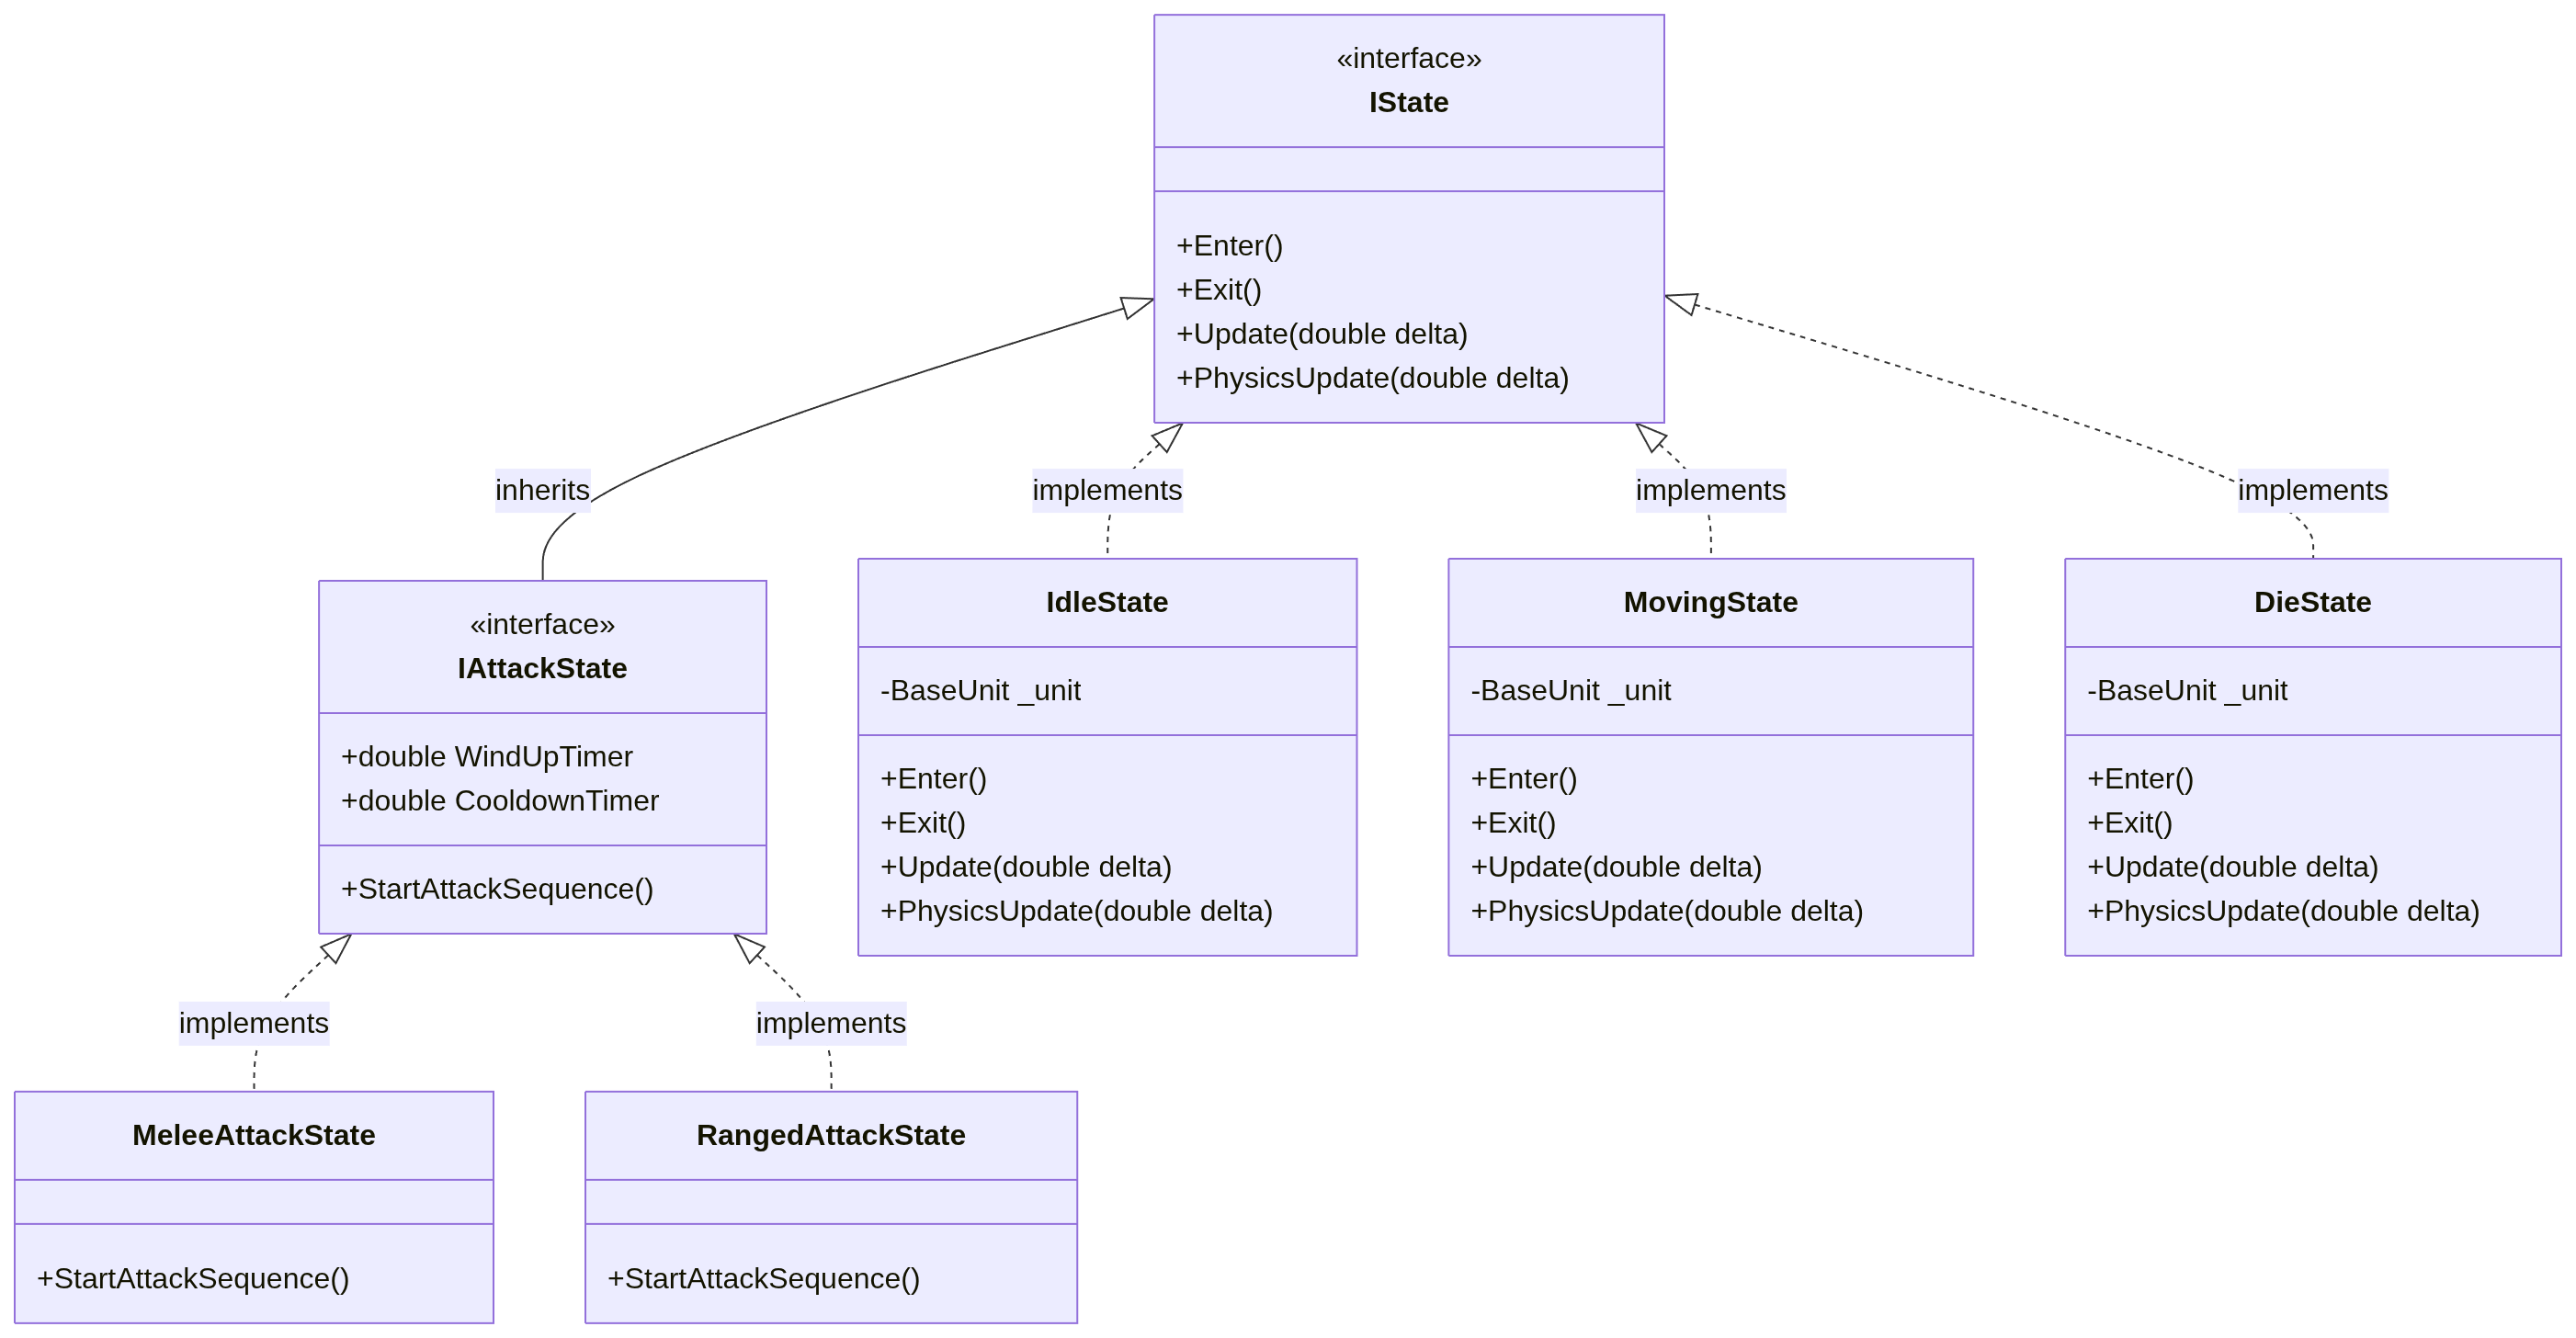
\includegraphics[width=0.9\textwidth]{ClassDiagram.png}
    \caption{Diagrama UML de clase ilustrând moștenirea interfeței IAttackState}
    \label{fig:uml_attack_state}
\end{figure}
% --------------------------------------

Execuția propriu-zisă a atacului este delegată claselor concrete care implementează această interfață:
\begin{itemize}
    \item \textbf{\texttt{MeleeAttackState}:} Implementează \texttt{IAttackState} și aplică daune directe prin intermediul componentei \textit{Hitbox}.
    \item \textbf{\texttt{RangedAttackState}:} Implementează \texttt{IAttackState} și se ocupă de instanțierea proiectilelor.
\end{itemize}


\section{Arhitectura Backend-ului (.NET 10)}
\label{sec:arhitectura_backend}

Serverul este organizat folosind o arhitectură stratificată (Layered Architecture), asigurând o separare clară între interfața API, logica de business și accesul la date.

Pentru gestionarea utilizatorilor și asigurarea securității datelor (hash-uirea parolelor, generarea de token-uri), sistemul backend integrează framework-ul \textit{ASP.NET Core Identity}\cite{aspnet_identity_docs}. Această soluție a fost aleasă deoarece oferă nativ o arhitectură robustă pentru autentificare și stocare securizată, compatibilă direct cu Entity Framework Core .

\begin{itemize}
    \item \textbf{Controllere:} Gestionează cererile HTTP și returnează răspunsuri formatate JSON.
    \item \textbf{Servicii:} Conțin logica centrală, cum ar fi \texttt{MatchmakingService}, care este injectat în controllere folosind mecanismul nativ de \textit{Dependency Injection} (DI) din .NET.
    \item \textbf{Entități:} Reprezintă structura datelor în cod și sunt mapate peste tabelele bazei de date.
\end{itemize}

Utilizarea DI permite un cuplaj slab între componente, facilitând testarea unitară și mock-uirea bazei de date sau a altor servicii externe.

\section{Modelarea Datelor (Baza de Date SQLite)}
\label{sec:database}

Baza de date constituie stratul de persistență al arhitecturii. Am ales SQLite pentru simplitatea sa (serverless) și performanța adecvată pentru un proiect aflat în stadiul de prototip și dezvoltare locală.

Interacțiunea cu baza de date este realizată prin \textbf{Entity Framework Core}, utilizând abordarea \textit{Code-First}. Aceasta ne permite să definim schema bazei de date direct prin clase C\#, generând ulterior migrațiile necesare.

Principalele entități modelate sunt:
\begin{itemize}
    \item \texttt{AspNetUsers:} Extinde utilizatorul standard Identity pentru a include atribute specifice jocului, precum cantitatea de aur (\textit{Gold}), punctele de experiență (\textit{XP}) și nivelul.
    \item \texttt{Decks:} Reprezintă seturile de unități configurate de jucător pentru luptă, având o relație de tip 1-la-N cu utilizatorul.
    \item \texttt{UnitUnlocks:} Gestionează colecția de unități deblocate de fiecare jucător, permițând o progresie controlată în joc.
\end{itemize}

\begin{figure}[htbp]
    \centering
    % \includegraphics[width=0.9\textwidth]{erd_diagram}
    \caption{Diagrama Entitate-Relație (ERD)}
    \label{fig:erd_diagram}
\end{figure}



% Capitolul 4: Algoritmi și Mecanici Principale
\chapter{Algoritmi și Mecanici Principale}
\label{ch:algoritmi}

Complexitatea unui joc de strategie asimetric nu constă doar în logica vizuală sau în randarea graficii din client, ci și în eficiența sistemelor decizionale distribuite și în orchestrarea backend-ului. Acest capitol detaliază și analizează algoritmii centrali și arhitecturile concurente care guvernează funcționarea sistemului, accent-ul se pune pe eficiența computațională, gestionarea stărilor partajate și thread-safety.

\section{Algoritmul de Matchmaking și Gestiunea Instanțelor}
\label{sec:matchmaking}

Pentru a facilita conectarea jucătorilor într-un mediu competitiv multiplayer asimetric, a fost dezvoltat un serviciu de cuplare, ce a fost implementat pe serverul backend ASP.NET Core sub forma unui singleton coordonat asincron (\texttt{MatchmakingService}).

Acest sistem nu numai că asigură simpla asociere a doi utilizatori din coada de așteptare ci și acționează ca un orchestrator de procese Godot, fiind responsabil de crearea și izolarea instanțelor de execuție ale serverului de joc dedicat.

\subsection{Logica de Funcționare: Evaluare Imediată}
Algoritmul de matchmaking este proiectat după șablonul de arhitectură \textit{Producer-Consumer}, utilizând cozi de așteptare concurente, complet decuplate de firele de execuție care deservesc cererile HTTP/WebSocket ale clienților. Fluxul algoritmic este orchestrat de o clasă ce extinde \texttt{BackgroundService} din .NET, rulând o buclă infinită non-blocantă reglată prin semnale asincrone.

Etapele exacte ale algoritmului sunt descrise în continuare:
\begin{enumerate}
    \item \textbf{Înregistrarea Cererii (Production):} Jucătorul transmite o cerere de alocare specificând rolul dorit (\texttt{PlayerRole.Attacker} sau \texttt{PlayerRole.Defender}). Serverul validează jetonul de autentificare, generează un tichet unic de identificare și introduce referința utilizatorului în coada specifică rolului ales.
    \item \textbf{Evaluarea Concurentă (Consumption):} Bucla de fundal a serviciului interoghează starea cozilor dedicate. Evaluarea nu utilizează un mecanism primitiv de tip \textit{busy-waiting} (care ar epuiza resursele CPU), ci este trezită de mecanisme de sincronizare asincrone atunci când ambele cozi înregistrează elemente active. Când este îndeplinită condiția de existență a cel puțin unui candidat în fiecare structură (\texttt{AttackerQueue} și \texttt{DefenderQueue}), algoritmul extrage simultan cele două entități.
    \item \textbf{Alocarea Instanței și Pornirea Procesului Headless:} După extragerea cu succes, algoritmul generează un identificator unic global de meci (\texttt{MatchId} de tip GUID). Pentru a asigura o validare autoritară a meciului și a preveni trișarea (\textit{cheat prevention}), backend-ul nu deleagă logica către unul dintre clienți, ci instanțiază un proces separat, complet izolat, rulând executabilul Godot în mod \textit{Headless} (fără interfață grafică) pe sistemul de operare gazdă Linux/Ubuntu.

          Lansarea procesului se realizează programatic prin utilizarea clasei \texttt{System.Diagnostics.Process}, transmițând parametrii de configurare direct prin argumente în linie de comandă (CLI Args):
          \begin{itemize}
              \item Identificatorul unic al meciului (\texttt{--match-id});
              \item Configurația pachetelor de unități normalizate (\texttt{--defender-deck} și \texttt{--attacker-deck});
              \item Datele de profil sincronizate ale utilizatorilor (nume, indici de avatar).
          \end{itemize}
    \item \textbf{Persistența și Handshake-ul:} Starea meciului și configurarea inițială sunt persistate în baza de date relațională SQLite prin intermediul contextului Entity Framework Core. Clienții aflați în faza de așteptare recepționează asincron modificarea stării tichetului propriu și adresa instanței dedicate de Godot, inițiind faza de conexiune directă (Handshake) prin protocolul de rețea de nivel transport.
\end{enumerate}

% ---------------------------------------------------------
% PLACEHOLDER PENTRU DIAGRAMA FLOW MATCHMAKING
\begin{figure}[htbp]
    \centering
    % 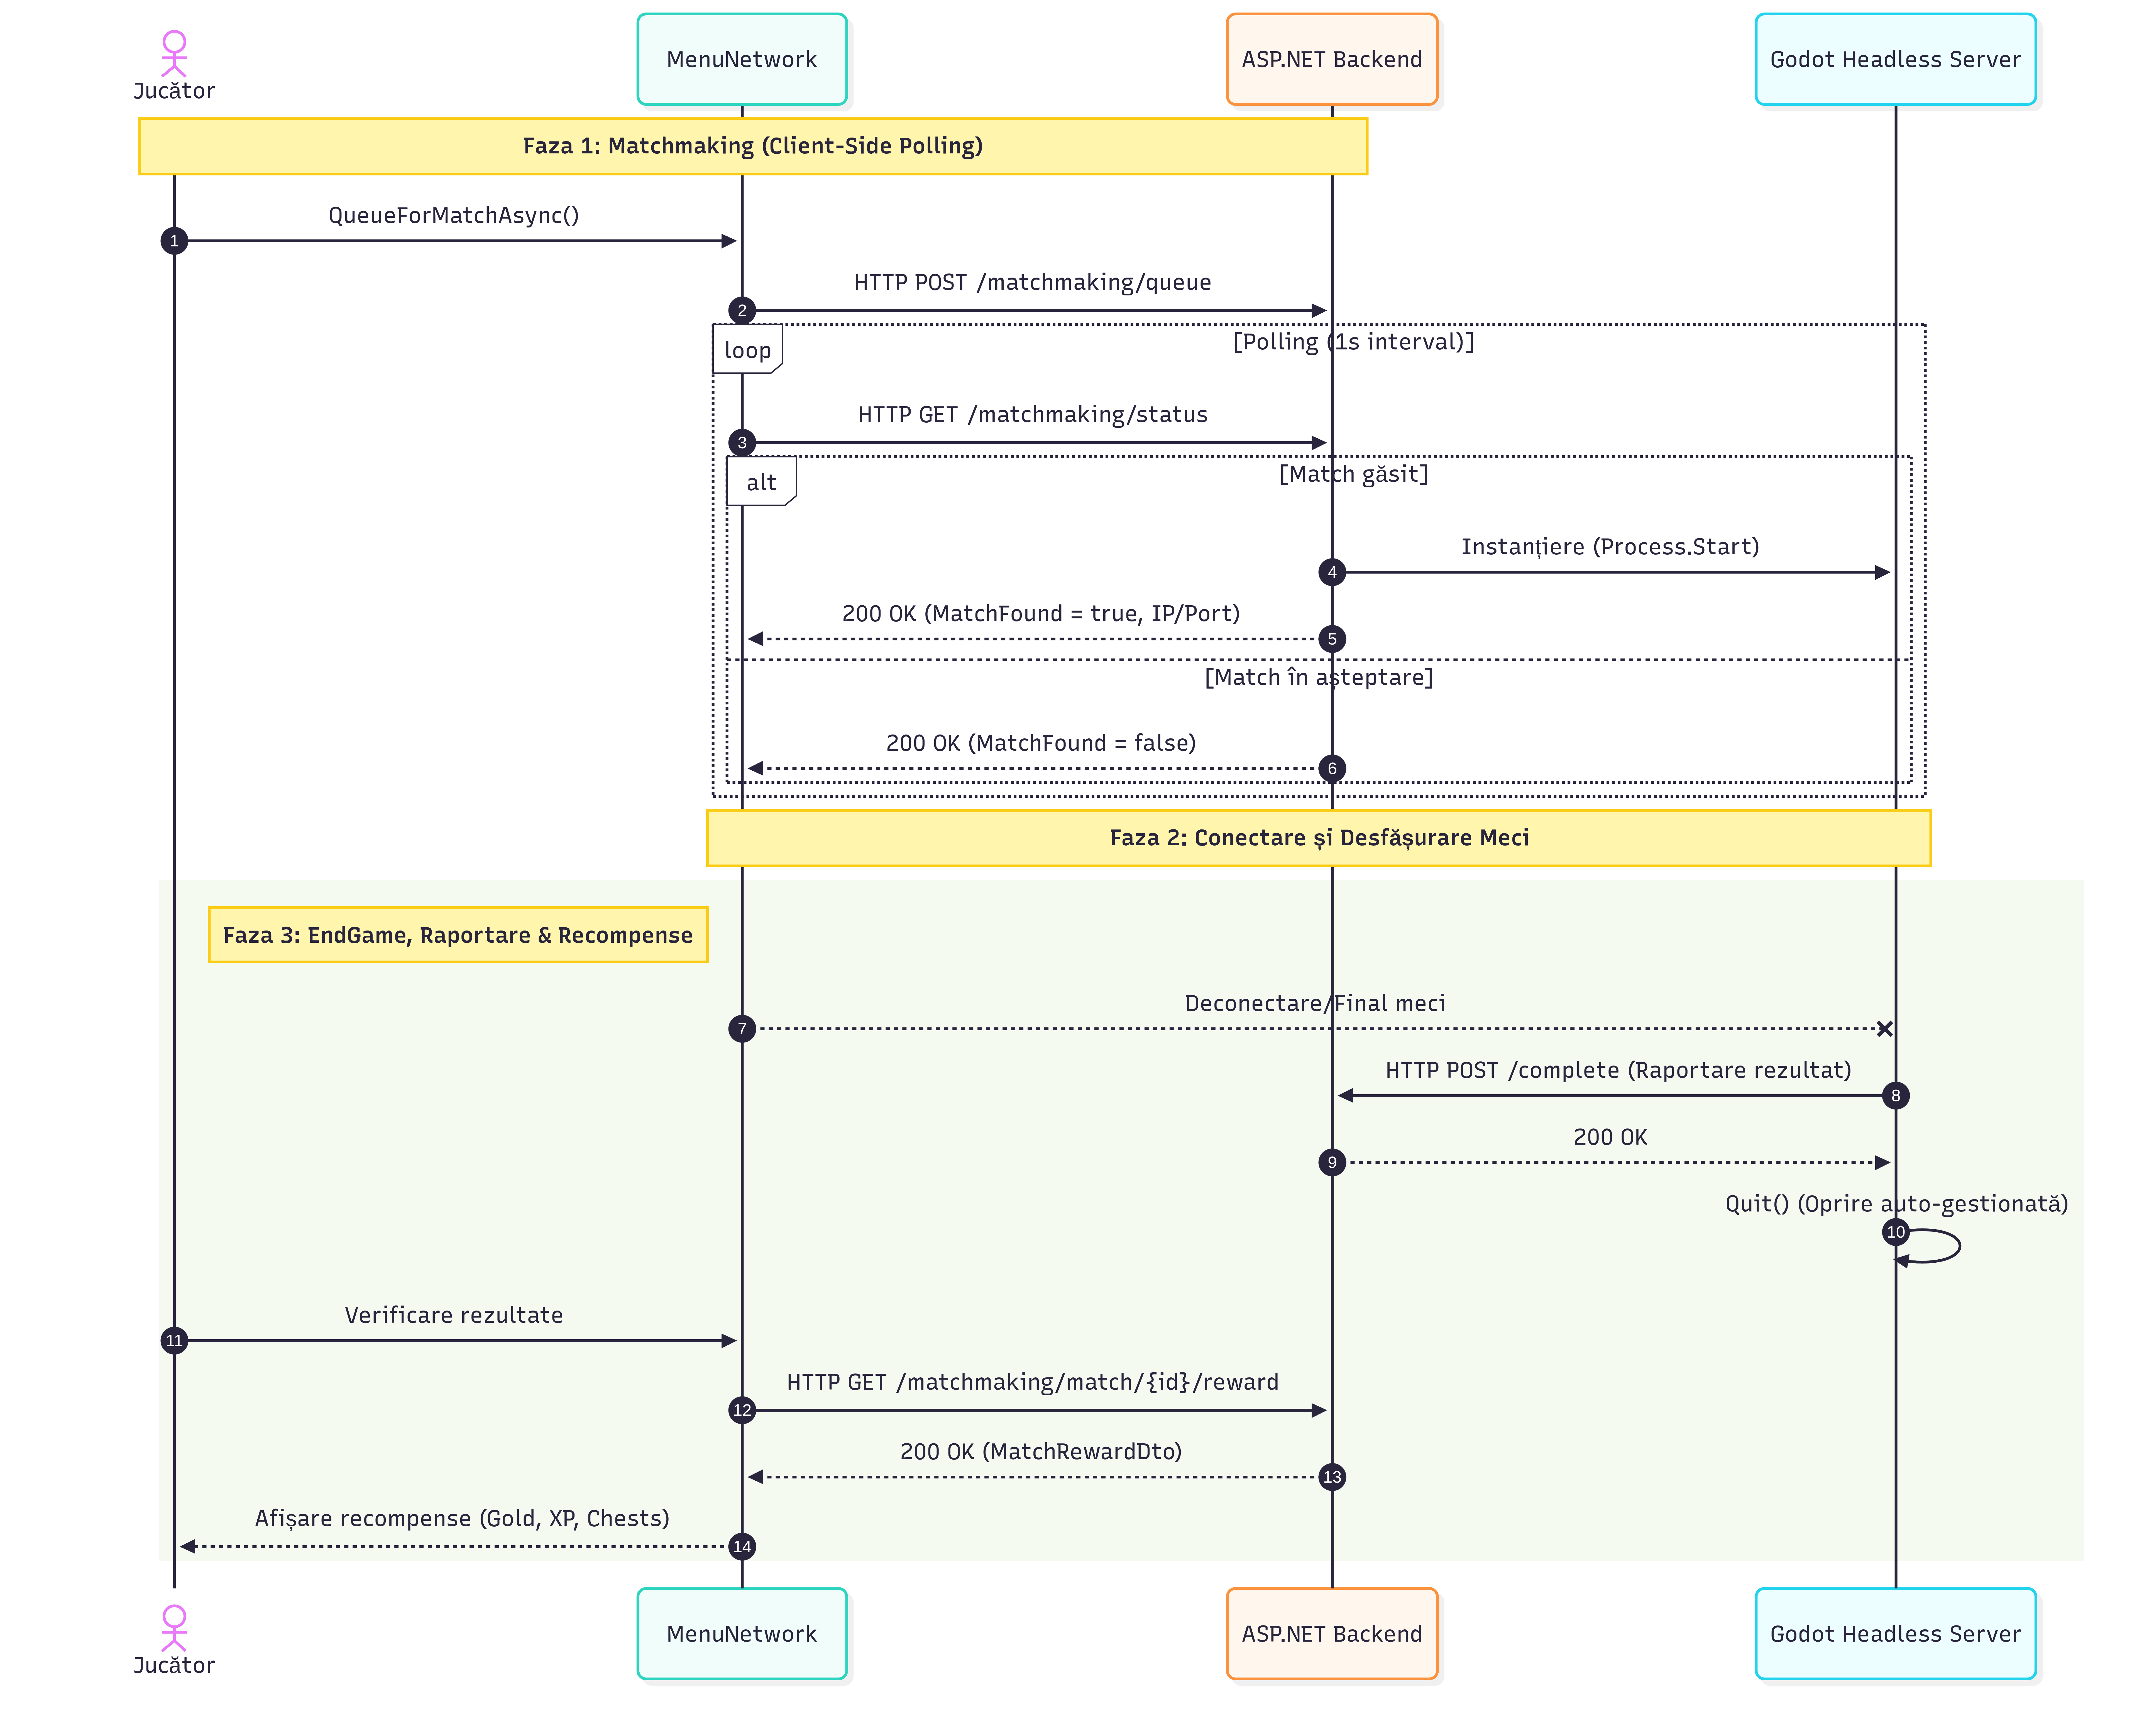
\includegraphics[width=\textwidth]{images/matchmaking-flow.png}
    \caption{Diagrama arhitecturală a sistemului de Matchmaking și ciclo-geneza serverului Headless}
    \label{fig:matchmaking_flow}
\end{figure}
% ---------------------------------------------------------

\subsection{Ciclul de Viață al Meciului și Toleranța la Eșec}
Odată instanțiat, serverul dedicat de Godot preia controlul absolut asupra simulării, funcționând după modelul \textit{Server-Authoritative}. Starea jocului (economia internă, timpul rămas și punctele de viață ale bazei) este calculată exclusiv pe server și propagată către clienți prin apeluri procedurale la distanță (RPC), prevenind astfel riscul de trișare prin manipularea memoriei locale a clientului.

Pentru a garanta robustețea sistemului în fața condițiilor reale de rețea, algoritmul de gestiune a meciului implementează multiple mecanisme de siguranță (Figura \ref{fig:matchmaking_flow}):
\begin{itemize}
    \item \textbf{Reziliența la Deconectări (Fault Tolerance):} În cazul pierderii conexiunii unui jucător, serverul nu oprește meciul imediat, ci inițiază o fereastră de grație asincronă (\texttt{Disconnect\-Grace\-Seconds}). Dacă utilizatorul nu reușește să restabilească o conexiune de nivel transport în intervalul de 30 de secunde, sistemul declară un abandon (\textit{forfeit}) în favoarea adversarului, asigurând fluiditatea experienței pentru jucătorii activi.
    \item \textbf{Comunicarea Inter-Procese (IPC):} La finalizarea condițiilor de victorie, instanța Headless comunică înapoi cu backend-ul ASP.NET Core printr-un apel HTTP autentificat. Raportarea rezultatului este validată folosind o cheie criptografică injectată în momentul ciclo-genezei (\texttt{MatchServerCallbackKey}), asigurând integritatea tranzacției de acordare a recompenselor (bani, experiență).
    \item \textbf{Prevenirea Proceselor Zombi:} În eventualitatea în care API-ul principal devine indisponibil și nu poate recepționa finalizarea meciului, instanța de joc folosește un \textit{safety timeout} local (\texttt{\_forceQuitTimer}). La expirarea acestuia, procesul de pe sistemul Linux se auto-termină forțat, prevenind astfel blocarea memoriei RAM (\textit{memory leaks}) și epuizarea resurselor infrastructurii (\textit{Resource Starvation}).
\end{itemize}

\subsection{Analiza Concurenței și Atomicitatea Tranzacțiilor}
Din punct de vedere computational, cozile de așteptare sunt implementate prin intermediul structurii de date \texttt{ConcurrentQueue<T>} furnizată de spațiul de nume \texttt{System.Collections.Concurrent}. Aceasta utilizează algoritmi lock-free bazați pe primitive atomice de tip \textit{Compare-And-Swap} (CAS), eliminând overhead-ul generat de blocajele tradiționale la nivel de kernel.

Operațiunile de adăugare (\texttt{Enqueue}) și extragere (\texttt{TryDequeue}) din cozile de așteptare se realizează în complexitate temporală constantă, amortizată $O(1)$. Prin urmare, algoritmul de împerechere prezintă o scalabilitate liniară în raport cu numărul de cereri concurente, limitarea fiind impusă exclusiv de resursele hardware (memorie și capacitate CPU pentru procesele Godot active în paralel).

Gestionarea concurenței este critică în momentul tranziției de la faza de cuplare la cea de instanțiere a procesului. Deoarece mai multe instanțe ale buclei asincrone sau cereri de anulare din partea utilizatorilor pot accesa simultan starea aceluiași tichet, operațiunile de scriere pe colecțiile de control ale stărilor active (\texttt{\_isProcessingRole}) sunt protejate prin secțiuni critice riguroase folosind mecanisme de excludere mutuală (\texttt{lock}).

Izolarea completă a logicii de simulare a jocului în procese \textit{Headless} distincte la nivelul nucleului Linux asigură că prăbușirea unei instanțe de joc din cauza unei erori de runtime nu afectează integritatea backend-ului ASP.NET Core sau a altor meciuri aflate în desfășurare, garantând o toleranță ridicată la eșec a întregului ecosistem.

\section{Sistemul Concurent de Sincronizare a Pachetului (Deck)}
\label{sec:deck_sync}

\subsection{Definirea Problemei și Abordarea Arhitecturală}
În aplicațiile interactive, manipularea rapidă a resurselor (ex. în proiectul curent: modificarea pachetelor de unități prin \textit{drag-and-drop}) implică apariția uonr provocări de sincronizare între client și server. Implementarea naivă ar fi recurgerea la apeluri HTTP sincrone, dar această abordare blochează interfața utilizatorului până la primirea răspunsului (Pessimistic Locking), ceea ce degradează semnificativ experiența vizuală.

Implementarea aleasă are în vedere principiul \textit{Server-Authoritative}, unde severul validează inputurile utilizatorului și deține informațiile finale despre starea jocului. Avantajele acestei abordări includ: fluiditatea interfeței, reducerea riscului de desincronizare și o experiență lipsită de sacadări vizuale.

\subsection{Coada Asincronă și Debouncing-ul Arhitectural}
Când utilizatorul solicită o mutare în pachetul de unități, componenta grafică deleagă noua configurație către serviciul (\texttt{DeckService}). Chiar dacă interfața vizuală rămâne interactivă și permite utilizatorului să efectueze noi mutări ale unităților (interacțiune non-blocantă), pachetul nu este actualizat instantaneu, ci așteaptă confirmarea serverului.

Pentru a preveni aglomerarea rețelei cu cereri HTTP la fiecare cadru (fenomen de \textit{spamming}) și a gestiona latența, serviciul implementează un mecanism de \textit{debouncing} cu excludere mutuală. Configurația solicitată este salvată într-un dicționar partajat (\texttt{\_pendingDeckByRole}), iar un identificator numeric de versiune (\texttt{\_latestVersionByRole}) este incrementat. Această operațiune este protejată de un blocaj \texttt{lock} (\textit{Thread Safety}).

O singură buclă asincronă (\texttt{ProcessSaveLoop}) este instanțiată pentru a iniția transmiterea datelor locale și a procesa modificările ce vin de pe server. Orice acțiune rapidă,  ulterioară a utilizatorului suprascrie pachetul ce este în așteptare pentru a fi actualizat pe server, fără a genera fire de execuție concurente.
% --- PLACEHOLDER DIAGRAMĂ DE SECVENȚĂ ---
\begin{figure}[htbp]
    \centering
    \includegraphics[width=0.85\textwidth]{images/async-debouncing-sync.png}
    \caption{Fluxul de sincronizare asincronă non-blocantă și anularea stărilor perimate}
    \label{fig:async_sync}
\end{figure}
% ----------------------------------------

\subsection{Validarea Răspunsurilor și Anularea Stărilor Precedente}
Deoarece cererile HTTP sunt procesate asincron, este prezent riscul ca răspunsurile de pe server să ajungă decalat (\textit{race conditions}). Sistemul rezolvă această problemă la finalizarea fiecărui apel (Figura \ref{fig:async_sync}).

Bucla evaluează dacă versiunea din momentul inițializării cererii coincide cu ultima versiune înregistrată la momentul primirii răspunsului (\texttt{IsLatestVersion}). Dacă utilizatorul a modificat pachetul de unități între timp, versiunea globală a fost deja actualizată(incrementată). În acest scenariu, răspunsul HTTP este considerat perimat (\textit{Stale Data}) și este ignorat, fără a declanșa vreo notificare pe ecran. Bucla extrage apoi noua configurație curentă a pachetului de unități și inițiază o nouă cerere către server.

Doar în momentul in care versiunile coincid, serviciul emite un semnal către clasa globală \texttt{GameState}, ce are ca scop actualizarea vizuală a interfeței grafice. Astfel, chiar dacă jucătorul a efectuat mutări/schimbări succesive rapide, UI-ul se va actualiza doar după rezultatul ultimei acțiuni, oferind o decuplare robustă și garantând că utilizatorul vede pe ecran numai starea confirmată de backend-ul \textit{ASP.NET Core}.

% Capitolul 5: Testare și Evaluare
\chapter{Testare și Evaluare}
\label{ch:testare}

Validarea soluției tehnice este un pas critic în dezvoltarea unui software academic riguros. În cadrul proiectului \textit{Farm Defense: Harvest Wars}, procesul de testare a fost împărțit în două direcții principale: testarea logică a backend-ului și evaluarea performanței clientului de joc.

\section{Testarea unitară a serviciilor backend}
% TODO: Descrie utilizarea xUnit/Moq pentru a testa MatchmakingService, DeckService, etc.

\section{Evaluarea performanței și testarea funcțională a clientului}
% TODO: Analizează FPS-ul, utilizarea memoriei în diferite scenarii de gameplay (ex: multe unități pe ecran).
% Menționează cum ai testat funcțional meciurile (ex: bot vs bot).


% Capitolul 6: Concluzii și Direcții Viitoare
\chapter{Concluzii și Direcții Viitoare}
\label{ch:concluzii}

\section{Concluzii asupra rezultatelor obținute}
% TODO: Rezumă ce ai realizat: arhitectură robustă, joc funcțional, etc.

\section{Propuneri de dezvoltare (Future Work)}
% TODO: Menționează ce ai vrea să adaugi: moduri noi de joc, trecerea la un protocol de rețea mai rapid (UDP/ENet), etc.


\printbibliography[heading=bibintoc]

\end{document}